\chapter{Bildvorverarbeitung}

Bevor nach der Aufnahme des Bildes nach Linien gesucht werden kann, muss das Bild entzerrt, gefiltert und binarisiert werden. 

\section{Bildentzerrung}

Der große Vorteil des Fischaugenobjektivs ist es, Bereiche in größerer Entfernung in alle Richtungen  wahrnehmen zu können. Jedoch ist es gerade für die Approximation der Fahrbahnmarkierungen zur Erstellung einer Weltkarte und der Regelung des Autos sinnvoll, dessen Verzerrung zurückzurechnen. Dazu wurde sich in \gls{glos:matlab} wie in~\ref{sec:kameramodell} beschrieben der OcamCalib-Toolbox bedient. Zuvor erfolgt außerdem eine Umwandlung in ein Graustufenbild, da wir die Farbinformation der Rohdaten nicht mit verarbeiten und sowohl die Toolbox als auch die Filter nur mit Schwarz-Weiß-Bildern, also einer Matrix deren Einträge die Helligkeitswerte der Pixel darstellt, arbeiten können. 

% Das ver- und entzerrte Bild nebeneinander
\begin{figure}[ht] % [htb]
  \centering
  \subfloat[][]{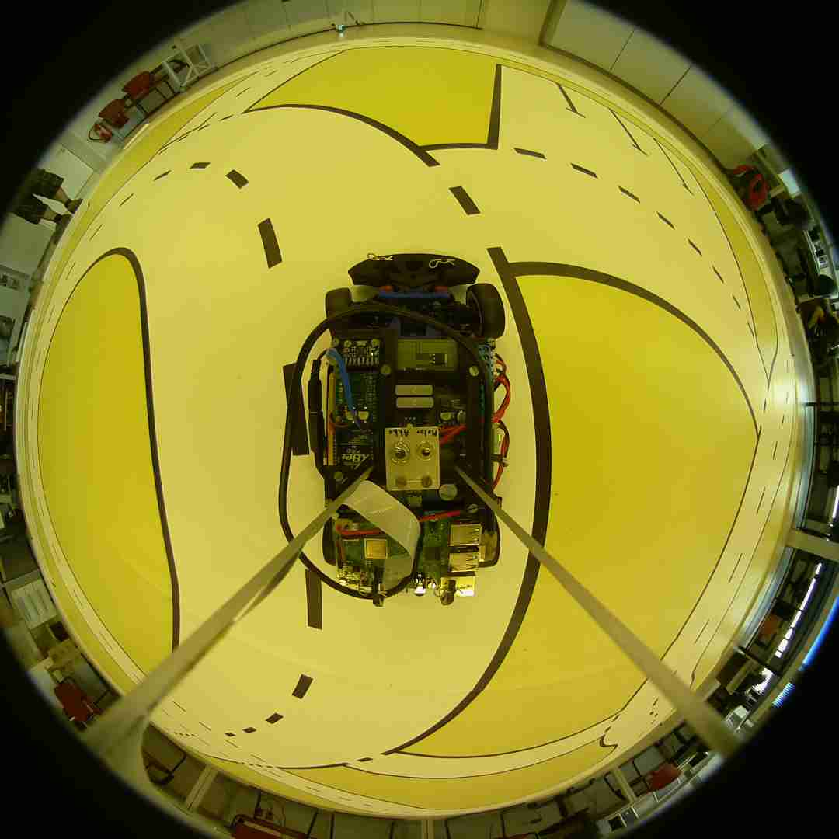
\includegraphics[width=0.45\textwidth]{bildvorverarbeitung_fischauge.png}}
  \qquad
  \subfloat[][]{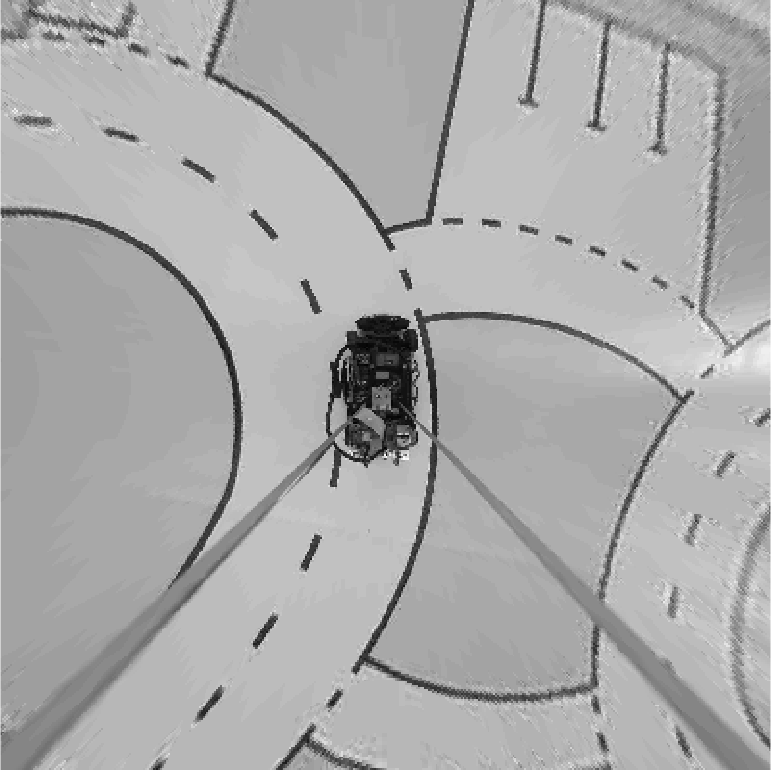
\includegraphics[width=0.45\textwidth]{bildvorverarbeitung_entzerrt.png}}
%  \includegraphics[width=0.9\textwidth]{bildvorverarbeitung_entzerren.png}
  \caption{verzerrtes Rohbild (a) und entzerrtes Graustufenbild (b) einer Momentaufnahme im Parcours}
\label{fig:bildvorverarbeitung_entzerren}
\end{figure} 

In~\ref{fig:bildvorverarbeitung_entzerren} ist zu sehen, wie das Bild original (links) und nach der Entzerrung (rechts) aussieht. Im entzerrten Bild fällt auf, dass zum Rand die Auflösung durch die Transformation immer schlechter wird. Daher haben wir den Bildausschnitt so weit begrenzt, sodass nach der Filterung die Linien noch akzeptabel erkennbar waren.

\section{Filterung}
Die Aufnahme soll nun wie in~\ref{sec:filter} beschrieben gefiltert werden, damit die Kanten (sprich: steile Übergänge von hellen zu dunklen Pixeln oder andersherum) hervorgehoben werden. Monotone Bildbereiche sollen dunkel bleiben. Würde man auf dem entzerrten Bild direkt eine Kantendetektion machen, erhielte man sehr viele Treffer, weil durch ganz normales Bildrauschen den Kantendetektor ansprechende Störungen enthalten sind. Das in Abbildung ~\ref{fig:bildvorverarbeitung_filtern} (a) dargestellte Filterergebnis wurde mit einem \gls{acr:log}-Filter erzielt. Er führt quasi zwei Filterungen mit einem Mal durch. Zum einen die gaußsche Glättung und den Laplace-Operator, der die Kanten hervorhebt. Mit entsprechend eingestellten Parameterwerten, ließen sich die eigentlich zwei an jeder Fahrbahnmarkierung entstandenen Kanten zu einer verwischen. Um wertvolle Rechenzeit bei der aufwändigen Filterung einzusparen, haben wir das Bild mit je einem eindimensionalen Filter in x- und in y-Richtung verarbeitet und anschließend die Filterergebnisse addiert. Das ist eine Alternative zu der in~\ref{sec:filter} beschriebenen Separierbarkeit und hat einen deutlich schnelleren Funktionsablauf ermöglicht. Das gefilterte Bild hat eine erstaunlich gute Qualität, mit dem sich wunderbar weiterarbeiten lässt.


% Das gefilterte und binarisierte Bild nebeneinander
\begin{figure}[hb] % [htb]
  \centering
  \subfloat[][]{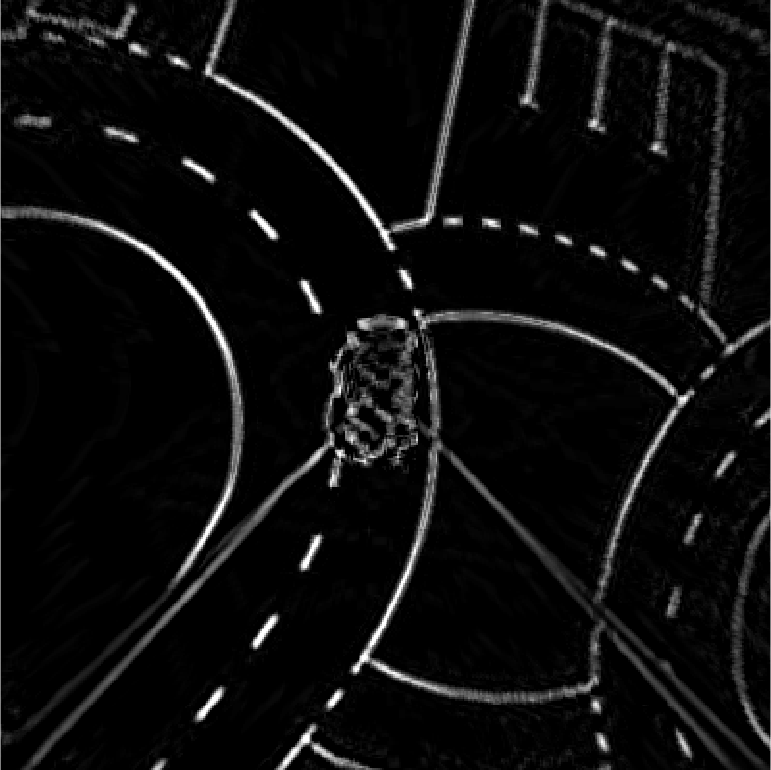
\includegraphics[width=0.45\textwidth]{bildvorverarbeitung_gefiltert.png}}
  \qquad
  \subfloat[][]{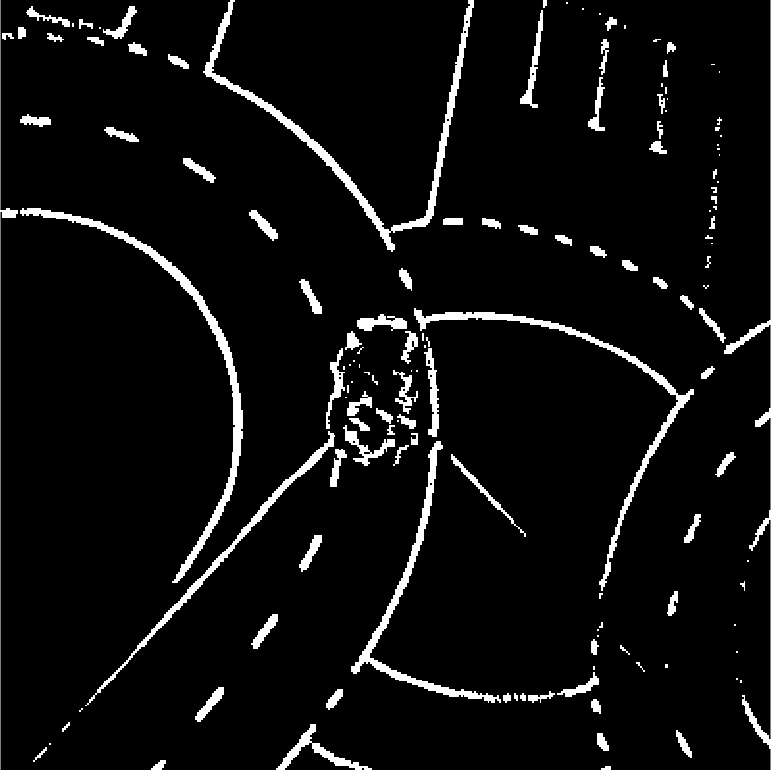
\includegraphics[width=0.45\textwidth]{bildvorverarbeitung_binarisiert.png}}
  \caption{gefiltertes (a) und anschließend binarisiertes Bild (b) einer Momentaufnahme im Parcours}
\label{fig:bildvorverarbeitung_filtern}
\end{figure} 

\section{Binarisierung}

Der Tresholdwert, welcher entscheidet, ob ein Pixel im binarisierten Bild den Wert \glqq \(0\)\grqq{} oder\glqq \(1\)\grqq{} erhält, wurde fest als Parameter eingestellt. Alle weiteren Bildverarbeitungsalgorithmen nehmen das binarisierte oder gefilterte Bild als Grundlage ihrer Berechnungen.